\section{Results}\label{sec:results}

This chapter presents the experimental results obtained from two groups of experiments. The transport protocol tests (T1-T6) and the codec configuration tests (C1-C9). Each group is evaluated across the five metrics system latency, packet loss rate, throughput, CPU usage on the sender, and visual quality. Interpretation and comparison are reserved for Chapter~\ref{sec:discussion}.

Transit latency data for C4 is unavailable due to a logging error during that test run. For the end-to-end result, the transit latency of C8 is used as a substitute for C4, as C8 had the closest matching throughput at 26.187~Mbps compared to C4's 26.267~Mbps, a difference of only 0.08~Mbps. Both tests also share GPU-accelerated encoding, making their network load profiles directly comparable. The C4 end-to-end result is marked with an asterisk (*) in Table~\ref{tab:end_codec_latency}.

For the unlimited bandwidth, a test of network was performed. The sender computer had a 112 Mbps Upload speed and the receiver had 148~Mbps Download speed. During the poor test, a value of 18 Mbps constrain on the Upload speed was used.

The transport protocol tests examine how the choice of transport layer protocol, encryption, and available bandwidth affect streaming performance. Table~\ref{tab:transport_duration} provides an overview of all six transport test configurations including the duration of test which matches the package number for packet loss calculations. 

\begin{table}[H]
    \centering
    \caption{Transport protocol test durations.}
    \label{tab:transport_duration}
    \begin{tabular}{@{}lccccc@{}}
        \toprule
        \textbf{Test} & \textbf{Protocol} & \textbf{Payload} & \textbf{Transcoding} & \textbf{Bandwidth} & \textbf{Duration} \\
        \midrule
        T1 & UDP & RTP  & Yes & Unlimited & 2:33 \\
        T2 & UDP & RTP  & No  & Unlimited & 2:08 \\
        T3 & UDP & SRTP & Yes & Unlimited & 2:49 \\
        T4 & TCP & RTP  & Yes & Unlimited & 1:57 \\
        T5 & UDP & RTP  & Yes & Poor      & 2:52 \\
        T6 & TCP & RTP  & Yes & Poor      & 1:25 \\
        \bottomrule
    \end{tabular}
\end{table}


The codec configuration tests examine how codec choice, resolution, and encoding hardware affect streaming performance. All tests used UDP - RTP transport with unlimited bandwidth, isolating codec-related variables from transport effects. Also take a look at Table~\ref{tab:camera_stream_config} for set values of the cameras that entered the computer and was passed along for the \textit{No transcoding} tests. Table~\ref{tab:codec_duration} provides an overview of all nine configurations. C1 served as the baseline configuration. As for the duration it gives a slight insight of how fast the car was driving as the test was completed on the same track each time. Worth noting is the fact that duration time is without the first 10 seconds dedicated to startup.

\begin{table}[H]
    \centering
    \caption{Codec configuration test durations.}
    \label{tab:codec_duration}
    \begin{tabular}{@{}lccccc@{}}
        \toprule
        \textbf{Test} & \textbf{Codec} & \textbf{Resolution} & \textbf{Transcoding} & \textbf{Encoding} & \textbf{Duration} \\
        \midrule
        C1 & H.264        & 1080p & Yes & CPU & 2:47 \\
        C2 & H.264        & 1080p & No  & \-- & 2:28 \\
        C3 & H.264        & 720p  & Yes & CPU & 2:46 \\
        C4 & H.264        & 1080p & Yes & GPU & 2:31 \\
        C5 & H.265        & 1080p & Yes & CPU & 2:15 \\
        C6 & H.265        & 1080p & No  & \-- & 2:26 \\
        C7 & H.265        & 720p  & Yes & CPU & 2:23 \\
        C8 & H.265        & 1080p & Yes & GPU & 2:27 \\
        C9 & MJPEG        & 1080p & Yes & CPU & 2:17 \\
        \bottomrule
    \end{tabular}
\end{table}



\subsection{System Latency}\label{subsec:system_latency}

The latency result is split up into multiple steps. Sender latency, Transit latency and lastly Receiver latency. Combined they give out a full end-to-end latency. All the latencies of the system were measured using timestamps at the sender and receiver. T1 and C1 served as the baseline configurations. Table~\ref{tab:send_transport_latency} summarises the mean, minimum, maximum and 95\% percentile of latency in sender for each transport test.

The no-transcode configurations (C2 and C6) have no sender pipeline stage and are therefore reported as N/A in the sender table. Table~\ref{tab:send_codec_latency} summarises the mean, minimum, maximum and 95\% percentile of latency in the sender pipeline for each codec test.

\textbf{Sender pipeline:}

\begin{table}[H]
    \centering
    \caption{Latency statistics for transport protocol tests for Sender pipeline.}\label{tab:send_transport_latency}
    \begin{tabular}{|l|l|c|c|c|c|}
    \hline
    \textbf{Test} & \textbf{Equipment} & \textbf{Mean [ms]} & \textbf{Min [ms]} & \textbf{Max [ms]} & \textbf{95p [ms]} \\
    \hline
    T1 & UDP RTP & 9.798 & 0.083 & 30.039 & 14.464\\
    \hline
    T2 & UDP RTP Passthrough & N/A & N/A & N/A & N/A  \\
    \hline
    T3 & UDP SRTP & 10.692 & 0.078 & 37.486 & 16.389 \\
    \hline
    T4 & TCP RTP & 9.984 & 0.086 & 25.219 & 14.799  \\
    \hline
    T5 & UDP RTP low bandwidth & 9.944 & 0.103 & 26.769 & 15.332\\
    \hline
    T6 & TCP RTP low bandwidth & 17.501 & 0.094 & 120.139 & 36.670 \\
    \hline
    \end{tabular}
\end{table}


\begin{table}[H]
    \centering
    \caption{Latency statistics for codec configuration tests for Sender pipeline.}\label{tab:send_codec_latency}
    \begin{tabular}{|l|l|c|c|c|c|}
    \hline
    \textbf{Test} & \textbf{Equipment} & \textbf{Mean [ms]} & \textbf{Min [ms]} & \textbf{Max [ms]} & \textbf{95p [ms]} \\
    \hline
    C1 & H.264 Baseline & 24.213 & 0.056 & 55.000 & 34.619\\
    \hline
    C2 & H.264 Passthrough & N/A & N/A & N/A & N/A  \\
    \hline
    C3 & H.264 720p & 23.118 & 0.681 & 45.819 & 30.377 \\
    \hline
    C4 & H.264 w/ GPU & 16.851 & 0.189 & 49.099 & 22.602  \\
    \hline
    C5 & H.265 & 26.807 & 0.122 & 100.533 & 50.045\\
    \hline
    C6 & H.265 Passthrough & N/A & N/A & N/A & N/A \\
    \hline
    C7 & H.265 720p & 29.295 & 0.046 & 87.836 & 55.596 \\
    \hline
    C8 & H.265 w/ GPU & 7.194 & 4.458 & 20.776 & 10.766 \\
    \hline
    C9 & MJPEG & 22.346 & 0.251 & 58.181 & 31.800  \\
    \hline
    \end{tabular}
\end{table}


\begin{figure}[H]
    \centering
    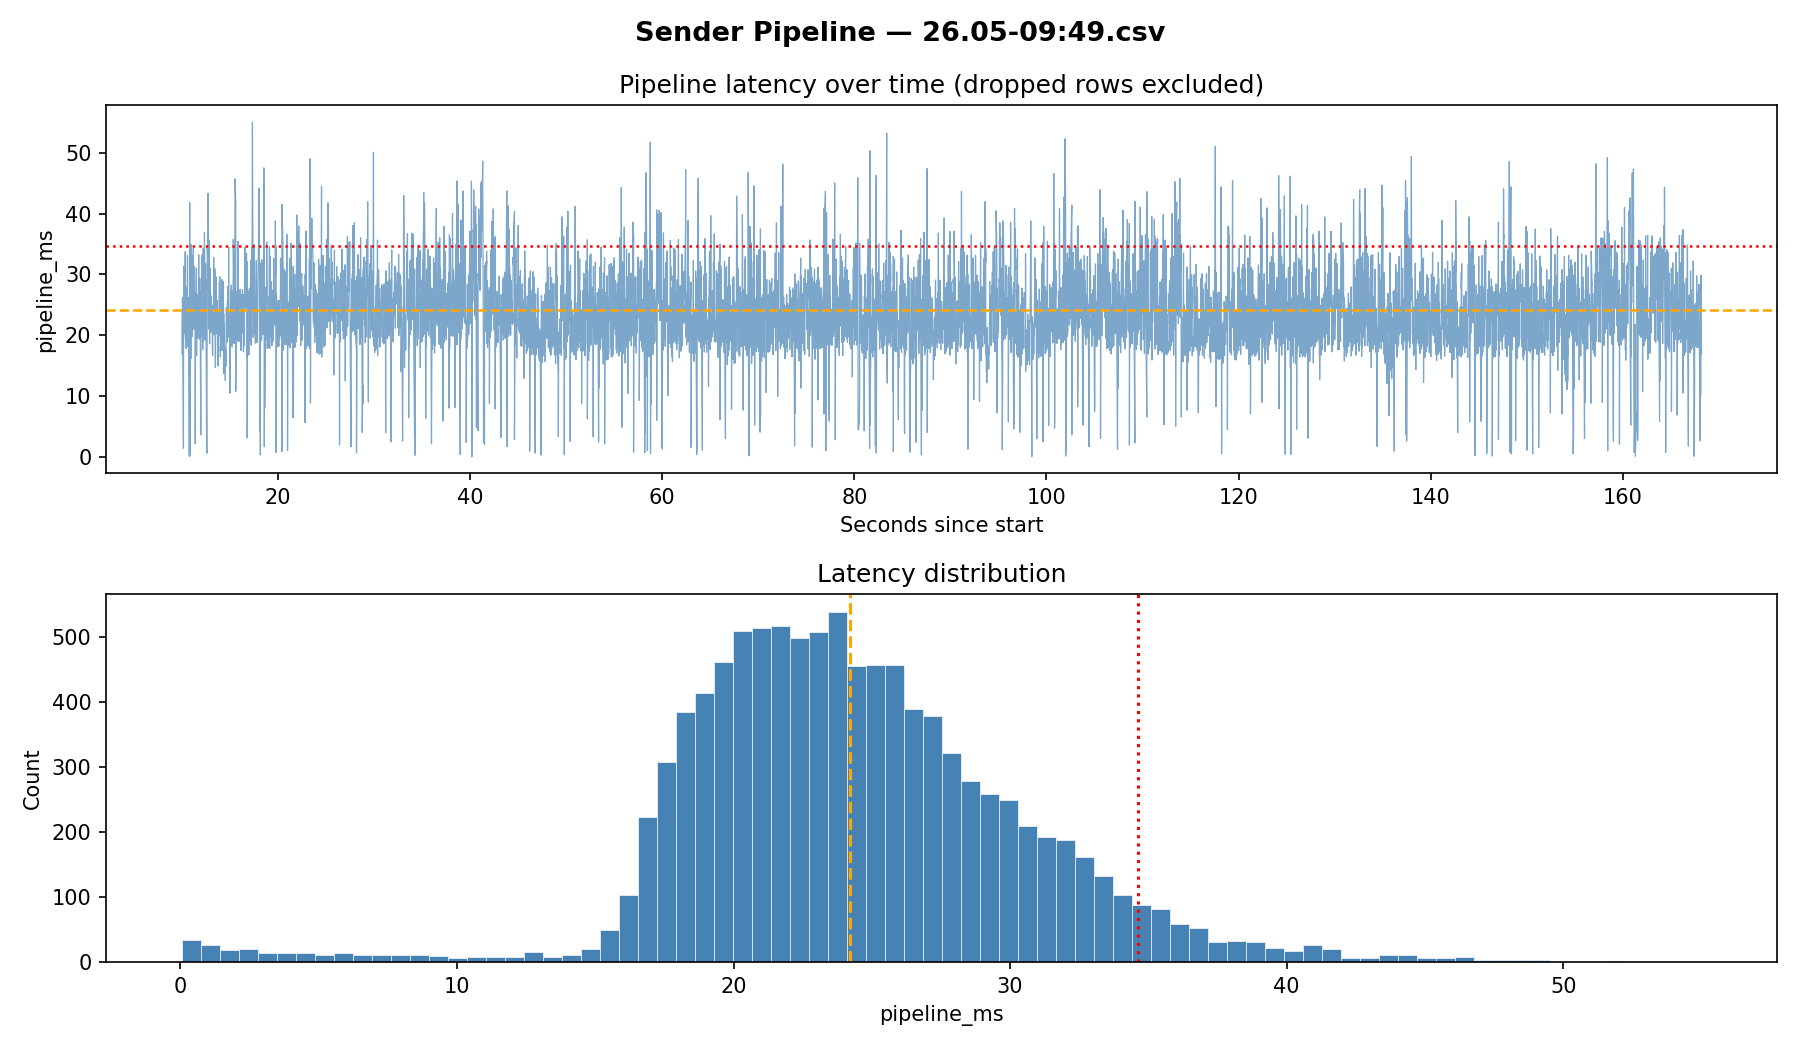
\includegraphics[width=0.95\textwidth]{Code/Analyzers/graphs/C1-26.05-09:49/sender_pipeline_26.05-09:49_analysis.png}
    \caption{Sender pipeline latency graph over time C1.}\label{fig:C1SenderLatency}
\end{figure}

\textbf{Transit:}

Transit latency is computed from timestamps on two separately clocked machines, the sender and the receiver. Before the experiments a clock offset check was completed, establishing a uncertainty of up to 7~ms between the clocks. Table~\ref{tab:transit_transport_raw} shows the raw, uncorrected values for the transport tests. The negative minimum values in the UDP tests are physically impossible and directly reflect the clock drift. The TCP tests  produced no negative values, as the higher inherent latency of TCP kept all measurements above zero.

\begin{table}[H]
    \centering
    \caption{Raw (uncorrected) latency statistics for transport protocol tests for Transit.}\label{tab:transit_transport_raw}
    \begin{minipage}{\linewidth}
    \centering
    \begin{tabular}{|l|l|c|c|c|c|}
    \hline
    \textbf{Test} & \textbf{Equipment} & \textbf{Mean [ms]} & \textbf{Min [ms]} & \textbf{Max [ms]} & \textbf{95p [ms]} \\
    \hline
    T1 & UDP RTP & 25.02 & \(-4.48\) & 530.89 & 86.36\\
    \hline
    T2 & UDP RTP Passthrough & 33.57 & \(-2.06\) & 537.08 & 109.24  \\
    \hline
    T3 & UDP SRTP & 27.51 & \(-5.26\) & 530.97 & 94.15 \\
    \hline
    T4\textsuperscript{*} & TCP RTP & 38.66 & 3.80 & 537.95 & 114.38  \\
    \hline
    T5 & UDP RTP low bandwidth & 35.35 & \(-2.17\) & 541.55 & 85.31\\
    \hline
    T6\textsuperscript{*} & TCP RTP low bandwidth & 9449.71 & 1940.78 & 35035.03 & 30190.97 \\
    \hline
    \end{tabular}
    \vspace{3pt}
    \par\noindent{\footnotesize \textsuperscript{*} TCP tests had no negative values and are identical to the offset-corrected table.}
    \end{minipage}
\end{table}


Since the clock offset is a constant bias across each test run, it can be removed by shifting every sample by the measured minimum, making the minimum 0~ms. This preserves all relative differences between measurements and keeps the results directly comparable across tests. Table~\ref{tab:transit_transport_latency} and Table~\ref{tab:transit_codec_latency} show the offset-corrected values used in the analysis. For the codec tests (C1--C9), all transit values were already positive under the same clock setup, so no correction was needed and the values are reported as measured.

\begin{table}[H]
    \centering
    \caption{Latency statistics for transport protocol tests for Transit}\label{tab:transit_transport_latency}
    \begin{tabular}{|l|l|c|c|c|c|}
    \hline
    \textbf{Test} & \textbf{Equipment} & \textbf{Mean [ms]} & \textbf{Min [ms]} & \textbf{Max [ms]} & \textbf{95p [ms]} \\
    \hline
    T1 & UDP RTP & 29.50 & 0.00 & 535.37 & 90.84\\
    \hline
    T2 & UDP RTP No Transcode & 35.63 & 0.00 & 539.14 & 111.30  \\
    \hline
    T3 & UDP SRTP & 32.77 & 0.00 & 536.23 & 99.41 \\
    \hline
    T4 & TCP RTP & 38.66 & 3.80 & 537.95 & 114.38  \\
    \hline
    T5 & UDP RTP low bandwidth & 37.52 & 0.00 & 543.72 & 87.48\\
    \hline
    T6 & TCP RTP low bandwidth & 9449.71 & 1940.78 & 35035.03 & 30190.97 \\
    \hline
    \end{tabular}
\end{table}


\begin{table}[H]
    \centering
    \caption{Latency statistics for codec configuration tests for Transit}\label{tab:transit_codec_latency}
    \begin{tabular}{|l|l|c|c|c|c|}
    \hline
    \textbf{Test} & \textbf{Equipment} & \textbf{Mean [ms]} & \textbf{Min [ms]} & \textbf{Max [ms]} & \textbf{95p [ms]} \\
    \hline
    C1 & H.264 Baseline & 31.98 & 0.73 & 579.72 & 102.41\\
    \hline
    C2 & H.264 No Transcode & 32.15 & 1.35 & 727.97 & 91.94  \\
    \hline
    C3 & H.264 720p & 44.71 & 0.59 & 2059.31 & 117.24 \\
    \hline
    C4 & H.264 w/ GPU & N/A & N/A & N/A & N/A  \\
    \hline
    C5 & H.265 & 40.94 & 2.61 & 551.56 & 129.33\\
    \hline
    C6 & H.265 No Transcode & 32.31 & 1.61 & 557.63 & 88.80 \\
    \hline
    C7 & H.265 720p & 40.30 & 2.73 & 819.00 & 112.86 \\
    \hline
    C8 & H.265 w/ GPU & 35.14 & 0.24 & 542.39 & 123.74 \\
    \hline
    C9 & MJPEG & 148.98 & 7.37 & 891.90 & 440.88  \\
    \hline
    \end{tabular}
\end{table}


\begin{figure}[H]
    \centering
    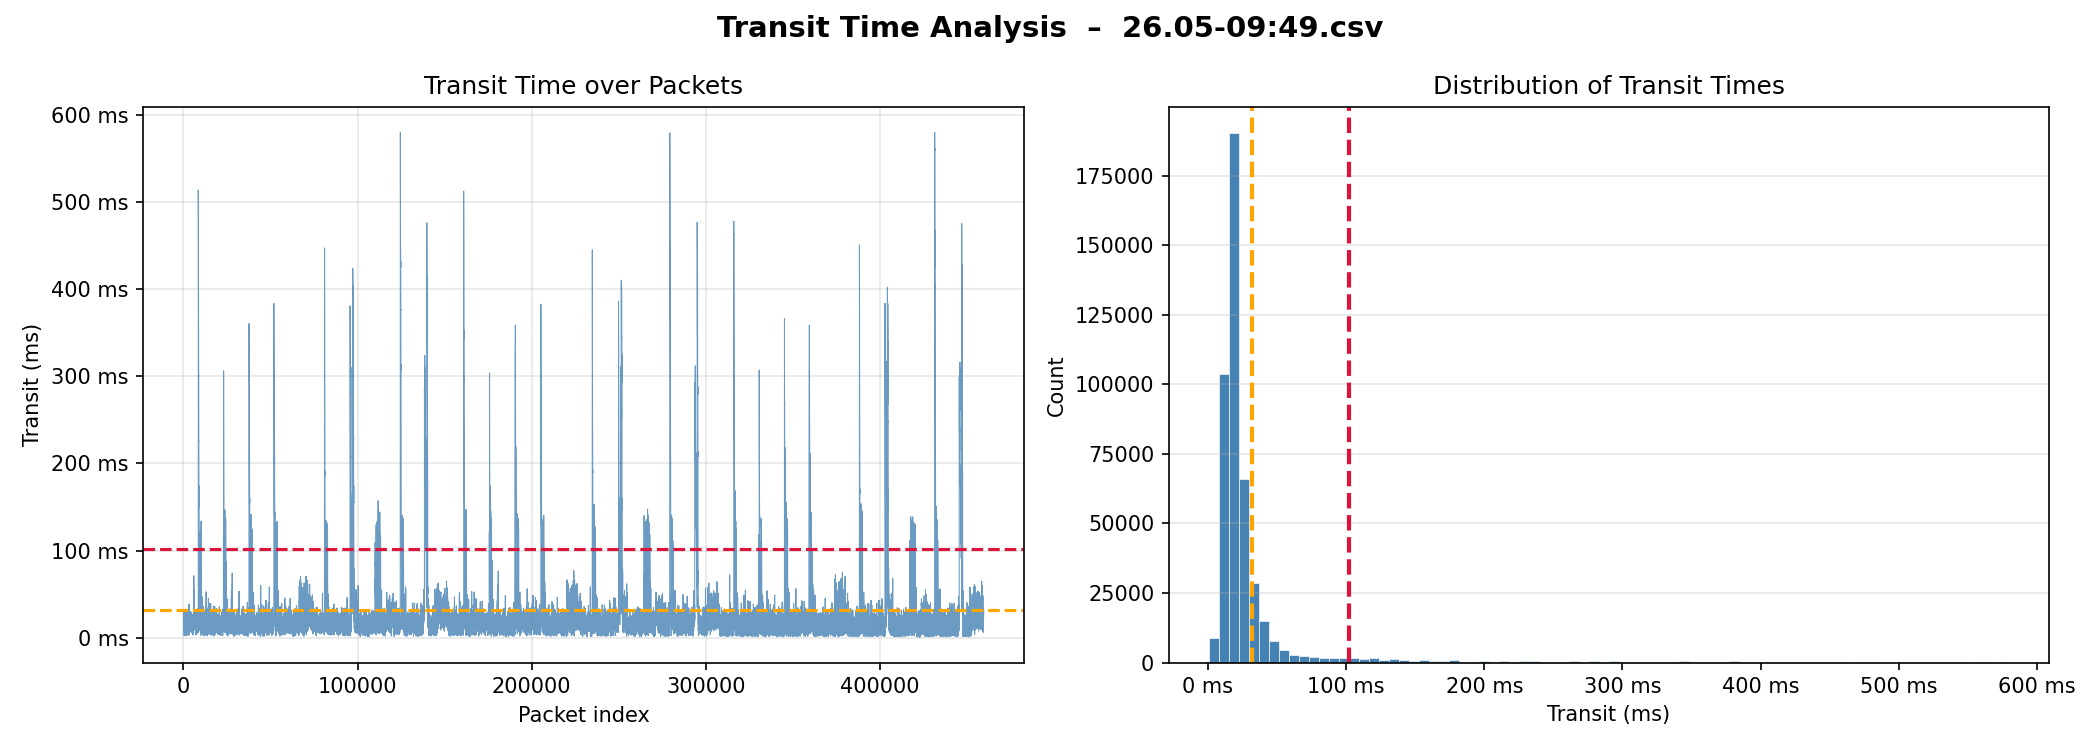
\includegraphics[width=0.95\textwidth]{Code/Analyzers/graphs/C1-26.05-09:49/transit_result_26.05-09:49_analysis.png}
    \caption{Transit latency graph over time for C1.}\label{fig:C1TransitLatency}
\end{figure}

\textbf{Receiver pipeline:}

\begin{table}[H]
    \centering
    \caption{Latency statistics for transport protocol tests for Receiver pipeline}\label{tab:receiver_transport_latency}
    \begin{tabular}{|l|l|c|c|c|c|}
    \hline
    \textbf{Test} & \textbf{Equipment} & \textbf{Mean [ms]} & \textbf{Min [ms]} & \textbf{Max [ms]} & \textbf{95p [ms]} \\
    \hline
    T1 & UDP RTP & 15.152 & 0.046 & 544.843 & 30.156\\
    \hline
    T2 & UDP RTP No Transcode & 14.772 & 0.044 & 488.626 & 42.351  \\
    \hline
    T3 & UDP SRTP & 16.162 & 0.046 & 542.424 & 36.931 \\
    \hline
    T4 & TCP RTP & 14.605 & 0.040 & 164.172 & 30.396  \\
    \hline
    T5 & UDP RTP low bandwidth & 10.858 & 0.079 & 68.871 & 29.761\\
    \hline
    T6 & TCP RTP low bandwidth & 37.151 & 0.036 & 642.592 & 101.650 \\
    \hline
    \end{tabular}
\end{table}


\begin{table}[H]
    \centering
    \caption{Latency statistics for codec configuration tests for Receiver pipeline.}\label{tab:rec_codec_latency}
    \begin{tabular}{|l|l|c|c|c|c|}
    \hline
    \textbf{Test} & \textbf{Equipment} & \textbf{Mean [ms]} & \textbf{Min [ms]} & \textbf{Max [ms]} & \textbf{95p [ms]} \\
    \hline
    C1 & H.264 Baseline & 19.220 & 0.036 & 514.203 & 38.809\\
    \hline
    C2 & H.264 No Transcode & 17.238 & 0.047 & 333.837 & 35.373  \\
    \hline
    C3 & H.264 720p & 15.373 & 0.037 & 1177.158 & 32.721 \\
    \hline
    C4 & H.264 w/ GPU & 17.140 & 0.042 & 480.279 & 35.535  \\
    \hline
    C5 & H.265 & 20.674 & 0.082 & 607.907 & 37.254\\
    \hline
    C6 & H.265 No Transcode & 24.454 & 0.038 & 559.511 & 48.209 \\
    \hline
    C7 & H.265 720p & 17.540 & 0.050 & 534.090 & 37.468 \\
    \hline
    C8 & H.265 w/ GPU & 22.461 & 0.059 & 530.366 & 40.949 \\
    \hline
    C9 & MJPEG & 21.817 & 0.048 & 541.738 & 49.279  \\
    \hline
    \end{tabular}
\end{table}


\begin{figure}[H]
    \centering
    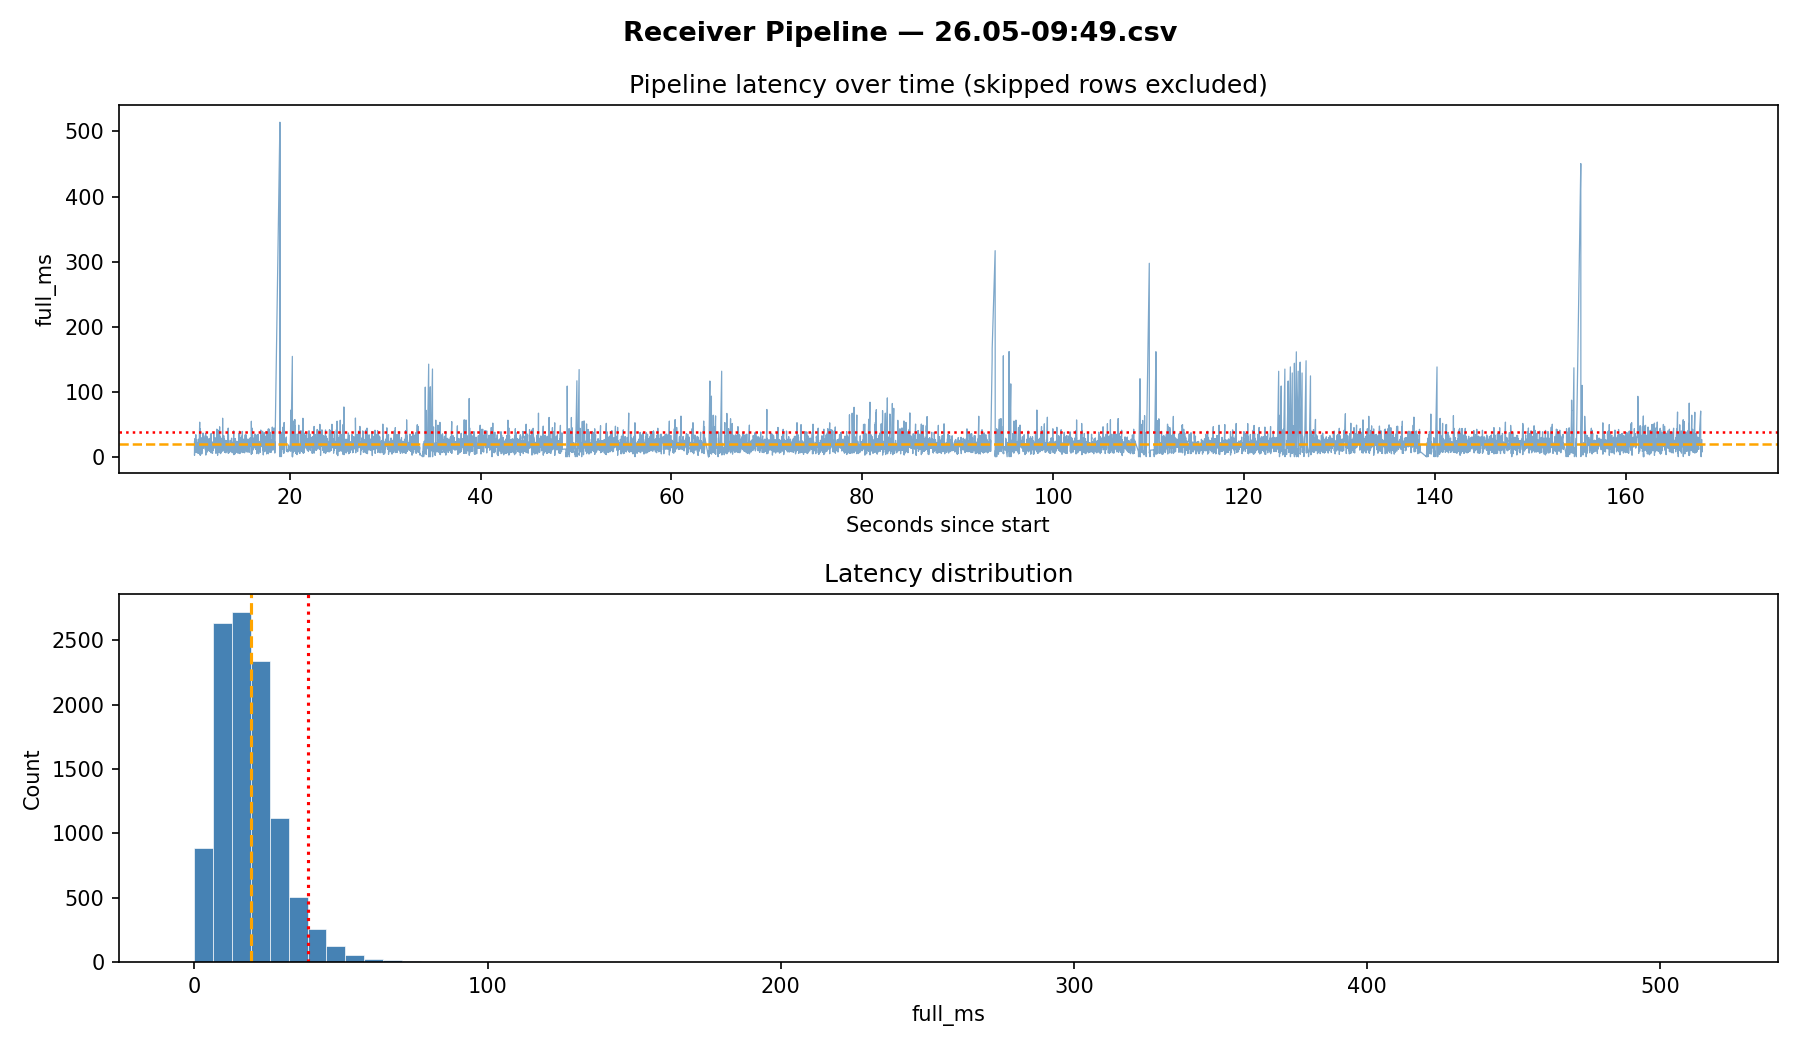
\includegraphics[width=0.95\textwidth]{Code/Analyzers/graphs/C1-26.05-09:49/receiver_pipeline_26.05-09:49_analysis.png}
    \caption{Receiver pipeline latency graph over time for C1.}\label{fig:C1ReceiverLatency}
\end{figure}

\textbf{End-to-End:}

End-to-end latency cannot be measured directly as the logged data does not allow matching a specific sender frame to the exact transit packet it was wrapped in and to the corresponding receiver decode, because each pipeline stage operates on different data formats as described in Chapter~\ref{chap:systemdesign}. The E2E figures are therefore approximate composites, obtained by independently summing each statistic across the three stages of sender pipeline, transit, and receiver pipeline. The mean composite is mathematically exact and the 95th-percentile composite is an upper-bound approximation summing the individual 95th percentiles assuming that all three stages simultaneously reach their highest latencies for the same frames, which is unlikely in practice and a conservative safety measure in the results. 

\begin{table}[H]
    \centering
    \caption{End-to-end latency statistics for transport protocol tests.}\label{tab:end_transport_latency}
    \begin{tabular}{|l|l|c|c|}
    \hline
    \textbf{Test} & \textbf{Equipment} & \textbf{Mean [ms]} & \textbf{95p [ms]} \\
    \hline
    T1 & UDP RTP & 54.450 & 135.460\\
    \hline
    T2 & UDP RTP Passthrough & 50.402 & 153.651  \\
    \hline
    T3 & UDP SRTP & 59.624 & 152.730 \\
    \hline
    T4 & TCP RTP & 63.249 & 159.575  \\
    \hline
    T5 & UDP RTP low bandwidth & 78.077 & 170.075\\
    \hline
    T6 & TCP RTP low bandwidth & 9504.362 & 30329.290 \\
    \hline
    \end{tabular}
\end{table}


\begin{table}[H]
    \centering
    \caption{End-to-end latency statistics for codec configuration experiment}\label{tab:end_codec_latency}
    \begin{minipage}{\linewidth}
    \centering
    \begin{tabular}{|l|l|c|c|c|c|}
    \hline
    \textbf{Test} & \textbf{Equipment} & \textbf{Mean [ms]} & \textbf{Min [ms]} & \textbf{Max [ms]} & \textbf{95p [ms]} \\
    \hline
    C1 & H.264 Baseline & 75.413 & 0.822 & 1148.923 & 175.838\\
    \hline
    C2 & H.264 No Transcode & 49.388 & 1.397 & 1061.807 & 127.313  \\
    \hline
    C3 & H.264 720p & 83.201 & 1.308 & 3282.287 & 180.338 \\
    \hline
    C4* & H.264 w/ GPU & 69.131 & 0.471 & 1071.768 & 181.877  \\
    \hline
    C5 & H.265 & 88.421 & 2.814 & 1260.000 & 216.629\\
    \hline
    C6 & H.265 No Transcode & 56.764 & 1.648 & 1117.141 & 137.009 \\
    \hline
    C7 & H.265 720p & 87.135 & 2.826 & 1440.926 & 205.924 \\
    \hline
    C8 & H.265 w/ GPU & 64.795 & 4.757 & 1093.532 & 175.455 \\
    \hline
    C9 & MJPEG & 193.143 & 7.669 & 1491.819 & 521.959  \\
    \hline
    \end{tabular}
    \vspace{3pt}
    \par\noindent{\footnotesize * Transit latency for C4 is substituted with the measured transit latency of C8, which had the nearest matching throughput (26.187 vs.\ 26.267~Mbps).}
    \end{minipage}
\end{table}


To better visualize where latency comes from, Figure~\ref{fig:latencyDistributionT1} and Figure~\ref{fig:latencyDistributionC1} is a diagram showing the latency distribution of T1 and C1, where the blocks are adjusted to symbolize the percentage they contribute to E2E latency.

%0.65 to 0.9 when adjusted
\begin{figure}[H]
    \centering
    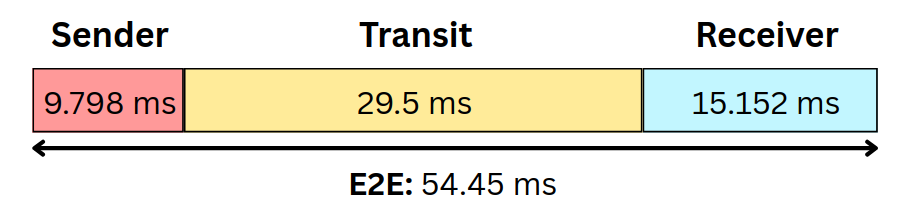
\includegraphics[width=0.65\textwidth]{Images/Results/E2ELatencyT1.png}
    \caption{End-to-end latency distribution for T1 UDP \- RTP, lab setup.}\label{fig:latencyDistributionT1}
\end{figure}

\begin{figure}[H]
    \centering
    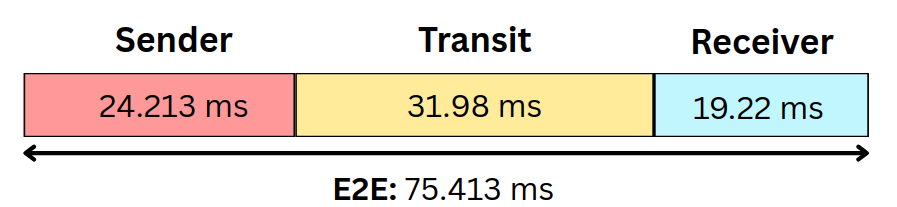
\includegraphics[width=0.65\textwidth]{Images/Results/E2ELatencyC1.png}
    \caption{End-to-end latency distribution for C1 H.264, moving experiment.}\label{fig:latencyDistributionC1}
\end{figure}

\subsection{Packet Loss Rate}\label{subsec:packet_loss}

Packet loss was calculated from RTP sequence numbers by logging every packet sent and every packet received, then matching the logs to determine how many packets sent by the sender were not received. For the entire experiment no excess packets were received that were not sent, indicating stable receiver logging. Packet loss data for C4 is unavailable due to the same logging error that affected transit data.

\begin{table}[H]
    \centering
    \caption{Packet loss statistics for transport protocol tests.}\label{tab:packetloss_transport}
    \begin{tabular}{|l|l|c|c|c|c|}
    \hline
    \textbf{Test} & \textbf{Equipment}  & \shortstack{\textbf{Sent}\\ \textbf{packets [n]}} & \shortstack{\textbf{Received}\\\textbf{packets [n]}} & \shortstack{\textbf{Packet}\\\textbf{loss [n]}} & \shortstack{\textbf{Packet}\\\textbf{loss [\%]}} \\
    \hline
    T1 & UDP RTP & 427,429 & 423,667 & 3,762 & 0.88\% \\
    \hline
    T2 & UDP RTP Passthrough & 255,418 & 254,574 & 844 & 0.33\% \\
    \hline
    T3 & UDP SRTP & 471,167 & 466,688 & 4,479 & 0.95\% \\
    \hline
    T4 & TCP RTP & 319,317 & 319,316 & 1 & 0.00\% \\
    \hline
    T5 & UDP RTP low bandwidth & 480,667 & 252,412 & 228,255 & 47.49\% \\
    \hline
    T6 & TCP RTP low bandwidth & 184,983 & 159,377 & 25,606 & 13.84\% \\
    \hline
    \end{tabular}
\end{table}


\begin{table}[H]
    \centering
    \caption{Packet loss statistics for codec configuration tests.}\label{tab:packetloss_codec}
    \begin{tabular}{|l|l|c|c|c|c|}
    \hline
    \textbf{Test} & \textbf{Equipment} & \shortstack{\textbf{Sent}\\ \textbf{packets [n]}} & \shortstack{\textbf{Received}\\\textbf{packets [n]}} & \shortstack{\textbf{Packet}\\\textbf{loss [n]}} & \shortstack{\textbf{Packet}\\\textbf{loss [\%]}} \\
    \hline
    C1 & H.264 Baseline & 463,464 & 459,661 & 3,803 & 0.82\% \\
    \hline
    C2 & H.264 No Transcode & 298,188 & 297,666 & 522 & 0.18\% \\
    \hline
    C3 & H.264 720p & 427,081 & 423,257 & 3,824 & 0.90\% \\
    \hline
    C4 & H.264 w/ GPU & N/A & N/A & N/A & N/A \\
    \hline
    C5 & H.265 & 95,090 & 94,412 & 678 & 0.71\% \\
    \hline
    C6 & H.265 No Transcode & 291,036 & 287,906 & 3,130 & 1.08\% \\
    \hline
    C7 & H.265 720p & 171,125 & 170,749 & 376 & 0.22\% \\
    \hline
    C8 & H.265 w/ GPU & 393,502 & 387,253 & 6,249 & 1.59\% \\
    \hline
    C9 & MJPEG & 905,545 & 838,721 & 66,824 & 7.38\% \\
    \hline
    \end{tabular}
\end{table}


\subsection{Throughput}\label{subsec:results_throughput}

Throughput was logged at the sender side and reflects the volume of encoded video data leaving the pipeline per second. Under unlimited bandwidth conditions (T1-T4), throughput reflects the natural output of the encoder with a bandwidth of over 100~Mbps. Under the poor bandwidth condition (T5 and T6), throughput is additionally constrained by the available capacity of 18~Mbps. The output measured includes the Tailscale wrapping adding a small percentage to the packets size, this is adjusted for in the constraint tests (T5 and T6) by adding a buffer at the constraint.

\begin{table}[H]
    \centering
    \caption{Throughput statistics for Transport experiment tests}\label{tab:throughput_transport}
    \begin{tabular}{|l|l|c|c|c|c|c|}
    \hline
    \textbf{Test} & \textbf{Equipment} & \shortstack{\textbf{Mean}\\ \textbf{[Mbps]}}  & \shortstack{\textbf{Min}\\ \textbf{[Mbps]}} & \shortstack{\textbf{Max}\\ \textbf{[Mbps]}} & \shortstack{\textbf{95p}\\ \textbf{[Mbps]}} & \shortstack{\textbf{Std. dev}\\ \textbf{[Mbps]}}\\
    \hline
    T1 & UDP RTP & 25.830 & 21.881 & 28.231 & 27.282 & 1.051\\
    \hline
    T2 & UDP RTP No Transcode & 24.907 & 19.726 & 29.467 & 28.156 & 2.993  \\
    \hline
    T3 & UDP SRTP & 26.069 & 21.311 & 29.707 & 27.977 & 1.390\\
    \hline
    T4 & TCP RTP & 26.148 & 23.518 & 27.921 & 27.645 & 1.195\\
    \hline
    T5 & UDP RTP low bandwidth & 18.259 & 0.000 & 19.377 & 19.027 & 2.936\\
    \hline
    T6 & TCP RTP low bandwidth & 18.691 & 14.863 & 19.057 & 18.968 & 0.861\\
    \hline
    \end{tabular}
\end{table}


\begin{table}[H]
    \centering
    \caption{Throughput statistics for codec configuration experiment tests}\label{tab:throughput_codec}
    \begin{tabular}{|l|l|c|c|c|c|c|}
    \hline
    \textbf{Test} & \textbf{Equipment} & \shortstack{\textbf{Mean}\\ \textbf{[Mbps]}} & \shortstack{\textbf{Min}\\ \textbf{[Mbps]}} & \shortstack{\textbf{Max}\\ \textbf{[Mbps]}} & \shortstack{\textbf{95p}\\ \textbf{[Mbps]}} & \shortstack{\textbf{Std. dev}\\ \textbf{[Mbps]}}\\
    \hline
    C1 & H.264 Baseline & 25.734 & 21.081 & 31.282 & 28.366 & 1.640\\
    \hline
    C2 & H.264 No Transcode & 24.973 & 20.572 & 30.348 & 26.748 & 1.454\\
    \hline
    C3 & H.264 720p & 25.591 & 19.348 & 29.272 & 28.521 & 1.763\\
    \hline
    C4 & H.264 w/ GPU & 26.267 & 19.394 & 34.360 & 30.623 & 2.798\\
    \hline
    C5 & H.265 & 8.573 & 3.110 & 26.997 & 18.863 & 4.446\\
    \hline
    C6 & H.265 No Transcode & 24.887 & 22.231 & 27.216 & 26.226 & 1.079\\
    \hline
    C7 & H.265 720p & 12.270 & 5.919 & 25.258 & 19.710 & 3.791\\
    \hline
    C8 & H.265 w/ GPU & 26.187 & 24.172 & 28.185 & 27.629 & 0.876\\
    \hline
    C9 & MJPEG & 80.867 & 53.250 & 120.931 & 107.205 & 15.083\\
    \hline
    \end{tabular}
\end{table}


\begin{figure}[H]
    \centering
    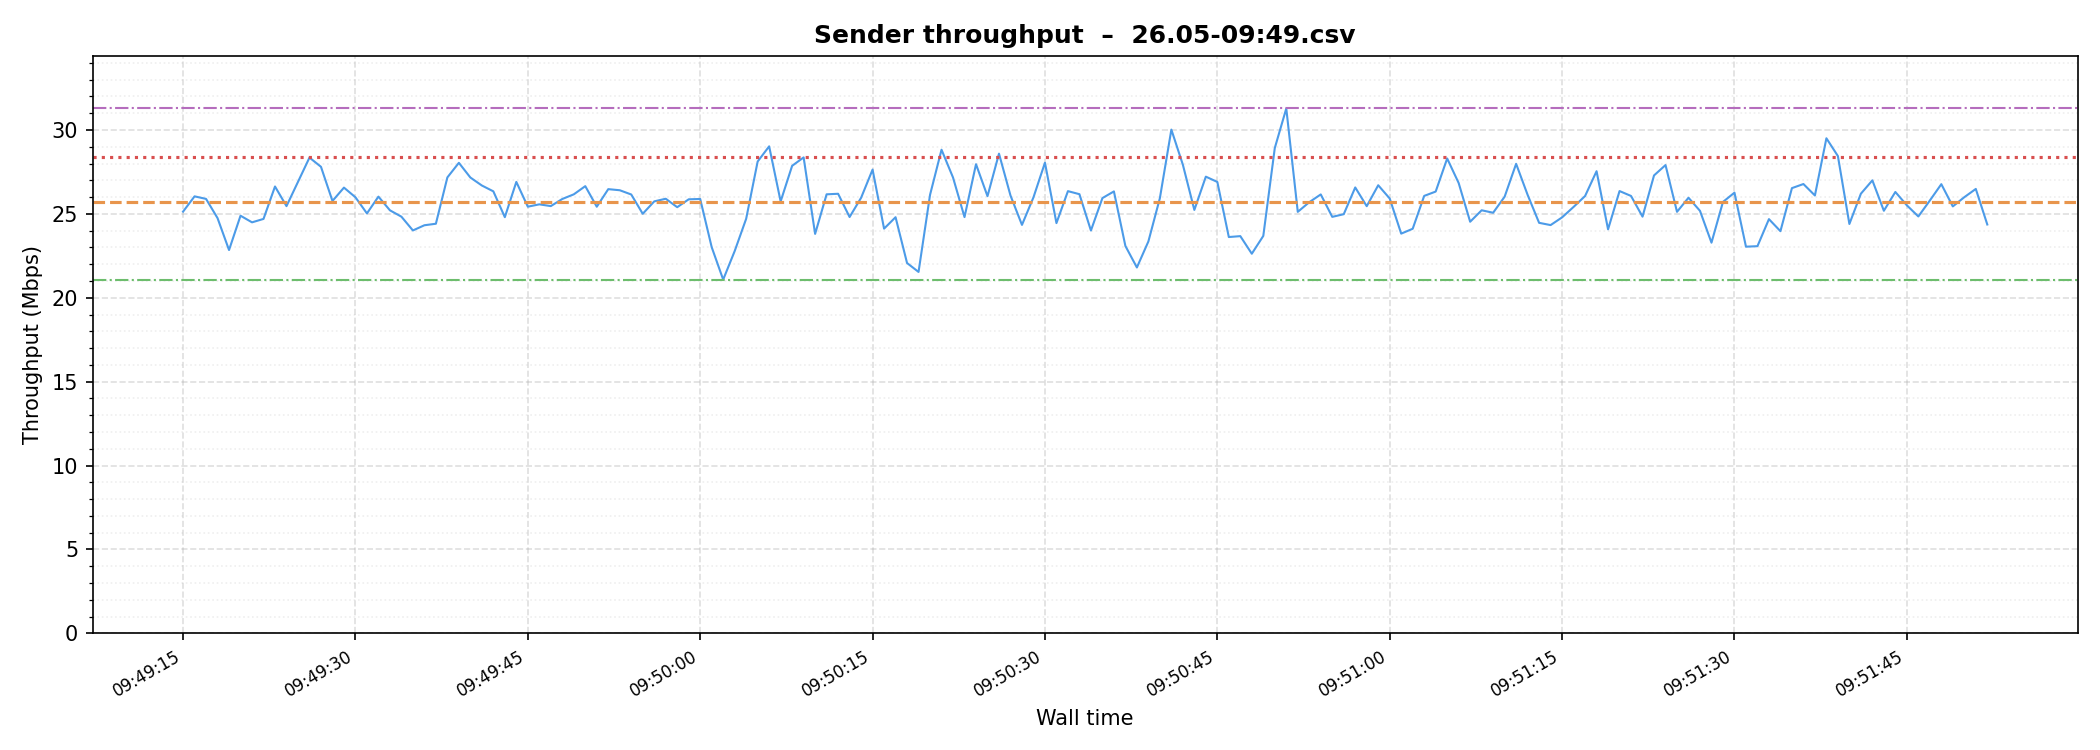
\includegraphics[width=0.95\textwidth]{Code/Analyzers/graphs/C1-26.05-09:49/throughput_26.05-09-49.png}
    \caption{Sender throughput graph over time for C1.}\label{fig:C1Throughput}
\end{figure}

\subsection{CPU Usage on Sender}\label{subsec:cpu_usage}

CPU usage was sampled at regular intervals during each test using the \texttt{sar} utility from the \texttt{sysstat} package. The values reported represent the total CPU load across all cores during the active streaming period. 
The no-transcode configurations C2 and C6 have no encoding step and are therefore reported as N/A.

\begin{table}[H]
    \centering
    \caption{Sender CPU usage statistics for Transport experiment tests}\label{tab:cpu_transport}
    \begin{tabular}{|l|l|c|c|c|c|c|}
    \hline
    \textbf{Test} & \textbf{Equipment} & \shortstack{\textbf{Mean}\\ \textbf{[\%]}} & \shortstack{\textbf{Min}\\ \textbf{[\%]}} & \shortstack{\textbf{Max}\\ \textbf{[\%]}} & \shortstack{\textbf{95p}\\ \textbf{[\%]}} & \shortstack{\textbf{Std. dev}\\ \textbf{[\%]}}\\
    \hline
    T1 & UDP RTP & 13.35 & 10.87 & 29.68 & 19.05 & 2.66\\
    \hline
    T2 & UDP RTP No Transcode & N/A & N/A & N/A & N/A & N/A\\
    \hline
    T3 & UDP SRTP & 14.29 & 11.87 & 19.99 & 17.58 & 1.64\\
    \hline
    T4 & TCP RTP & 13.80 & 11.36 & 17.02 & 16.24 & 1.15\\
    \hline
    T5 & UDP RTP low bandwidth & 13.25 & 11.36 & 19.34 & 15.02 & 1.04\\
    \hline
    T6 & TCP RTP low bandwidth & 29.91 & 11.17 & 51.67 & 46.01 & 11.70\\
    \hline
    \end{tabular}
\end{table}


\begin{table}[H]
    \centering
    \caption{Sender CPU usage statistics for codec configuration tests.}\label{tab:cpu_codec}
    \begin{tabular}{|l|l|c|c|c|c|c|}
    \hline
    \textbf{Test} & \textbf{Equipment} & \shortstack{\textbf{Mean}\\ \textbf{[\%]}} & \shortstack{\textbf{Min}\\ \textbf{[\%]}} & \shortstack{\textbf{Max}\\ \textbf{[\%]}} & \shortstack{\textbf{95p}\\ \textbf{[\%]}} & \shortstack{\textbf{Std. dev}\\ \textbf{[\%]}}\\
    \hline
    C1 & H.264 Baseline & 26.92 & 23.72 & 35.31 & 29.50 & 1.68\\
    \hline
    C2 & H.264 Passthrough & N/A & N/A & N/A & N/A & N/A\\
    \hline
    C3 & H.264 720p & 20.38 & 18.76 & 24.57 & 21.81 & 0.90\\
    \hline
    C4 & H.264 w/ GPU & 12.08 & 10.06 & 18.03 & 16.71 & 1.69\\
    \hline
    C5 & H.265 & 64.23 & 23.45 & 87.46 & 81.48 & 13.44\\
    \hline
    C6 & H.265 Passthrough & N/A & N/A & N/A & N/A & N/A\\
    \hline
    C7 & H.265 720p & 68.22 & 52.44 & 82.84 & 78.09 & 6.46\\
    \hline
    C8 & H.265 w/ GPU & 5.90 & 5.12 & 9.19 & 6.45 & 0.51\\
    \hline
    C9 & MJPEG & 17.26 & 14.38 & 24.46 & 20.30 & 1.78\\
    \hline
    \end{tabular}
\end{table}


\begin{figure}[H]
    \centering
    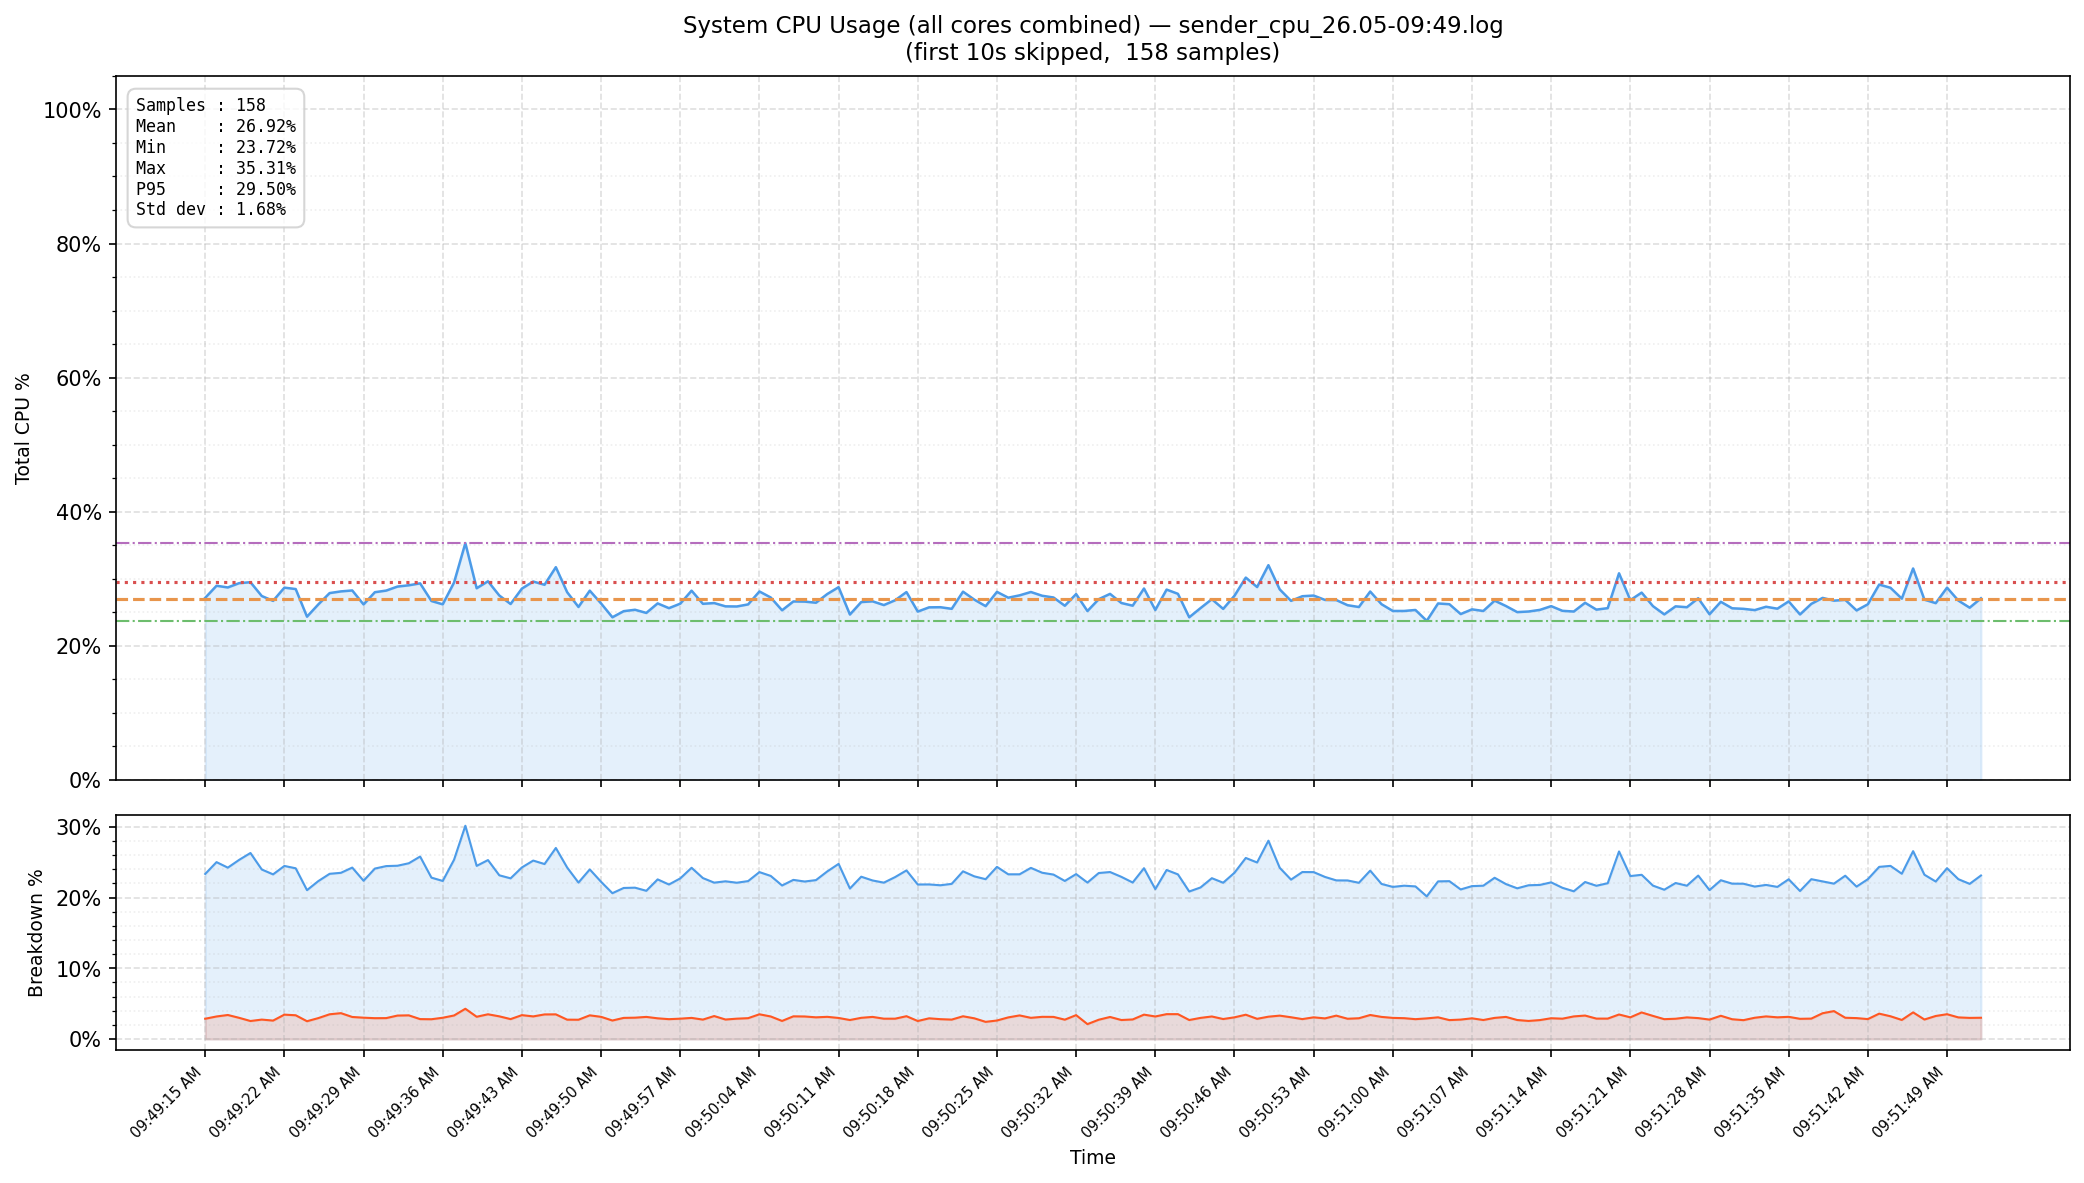
\includegraphics[width=0.95\textwidth]{Code/Analyzers/graphs/C1-26.05-09:49/sender_cpu_26.05-09:49_analysis.png}
    \caption{Sender CPU usage graph over time for C1.}\label{fig:C1CPU}
\end{figure}

\subsection{Visual Quality}\label{subsec:visual_quality}

Visual quality was assessed on captured frames using the BRISQUE no-reference image quality metric. Lower BRISQUE scores indicate better perceptual quality. Individual measurements were done per camera and the scores are aggregated across all three cameras per test.

\begin{table}[H]
    \centering
    \caption{BRISQUE visual quality statistics for Transport experiment tests (lower score = better quality)}\label{tab:quality_transport}
    \begin{tabular}{|l|l|c|c|c|c|}
    \hline
    \textbf{Test} & \textbf{Equipment} & \shortstack{\textbf{Mean}\\ \textbf{[score]}} & \shortstack{\textbf{Min}\\ \textbf{[score]}} & \shortstack{\textbf{Max}\\ \textbf{[score]}} & \shortstack{\textbf{95p}\\ \textbf{[score]}}\\
    \hline
    T1 & UDP RTP & 34.54 & 12.75 & 51.79 & 44.36\\
    \hline
    T2 & UDP RTP No Transcode & 13.70 & 4.35 & 82.72 & 21.58\\
    \hline
    T3 & UDP SRTP & 36.16 & 16.46 & 54.89 & 48.18\\
    \hline
    T4 & TCP RTP & 27.51 & 15.26 & 39.94 & 33.98\\
    \hline
    T5 & UDP RTP low bandwidth & 37.88 & 12.20 & 60.76 & 48.04\\
    \hline
    T6 & TCP RTP low bandwidth & 28.27 & 16.72 & 42.82 & 34.63\\
    \hline
    \end{tabular}
\end{table}


\begin{table}[H]
    \centering
    \caption{BRISQUE visual quality statistics for codec configuration tests.}\label{tab:quality_codec}
    \begin{tabular}{|l|l|c|c|c|c|}
    \hline
    \textbf{Test} & \textbf{Equipment} & \shortstack{\textbf{Mean}\\ \textbf{[score]}} & \shortstack{\textbf{Min}\\ \textbf{[score]}} & \shortstack{\textbf{Max}\\ \textbf{[score]}} & \shortstack{\textbf{95p}\\ \textbf{[score]}}\\
    \hline
    C1 & H.264 Baseline & 36.72 & 15.92 & 93.00 & 54.99\\
    \hline
    C2 & H.264 Passthrough & 29.90 & 12.19 & 49.83 & 38.59\\
    \hline
    C3 & H.264 720p & 30.04 & 8.04 & 108.05 & 67.73\\
    \hline
    C4 & H.264 w/ GPU & 43.48 & 27.20 & 106.65 & 54.10\\
    \hline
    C5 & H.265 & 33.13 & 18.91 & 110.90 & 46.18\\
    \hline
    C6 & H.265 Passthrough & 17.64 & 0.45 & 69.12 & 36.94\\
    \hline
    C7 & H.265 720p & 20.02 & 5.47 & 91.52 & 32.82\\
    \hline
    C8 & H.265 w/ GPU & 33.12 & 13.00 & 102.10 & 42.02\\
    \hline
    C9 & MJPEG & 40.00 & 24.92 & 100.94 & 52.76\\
    \hline
    \end{tabular}
\end{table}


\begin{figure}[H]
    \centering
    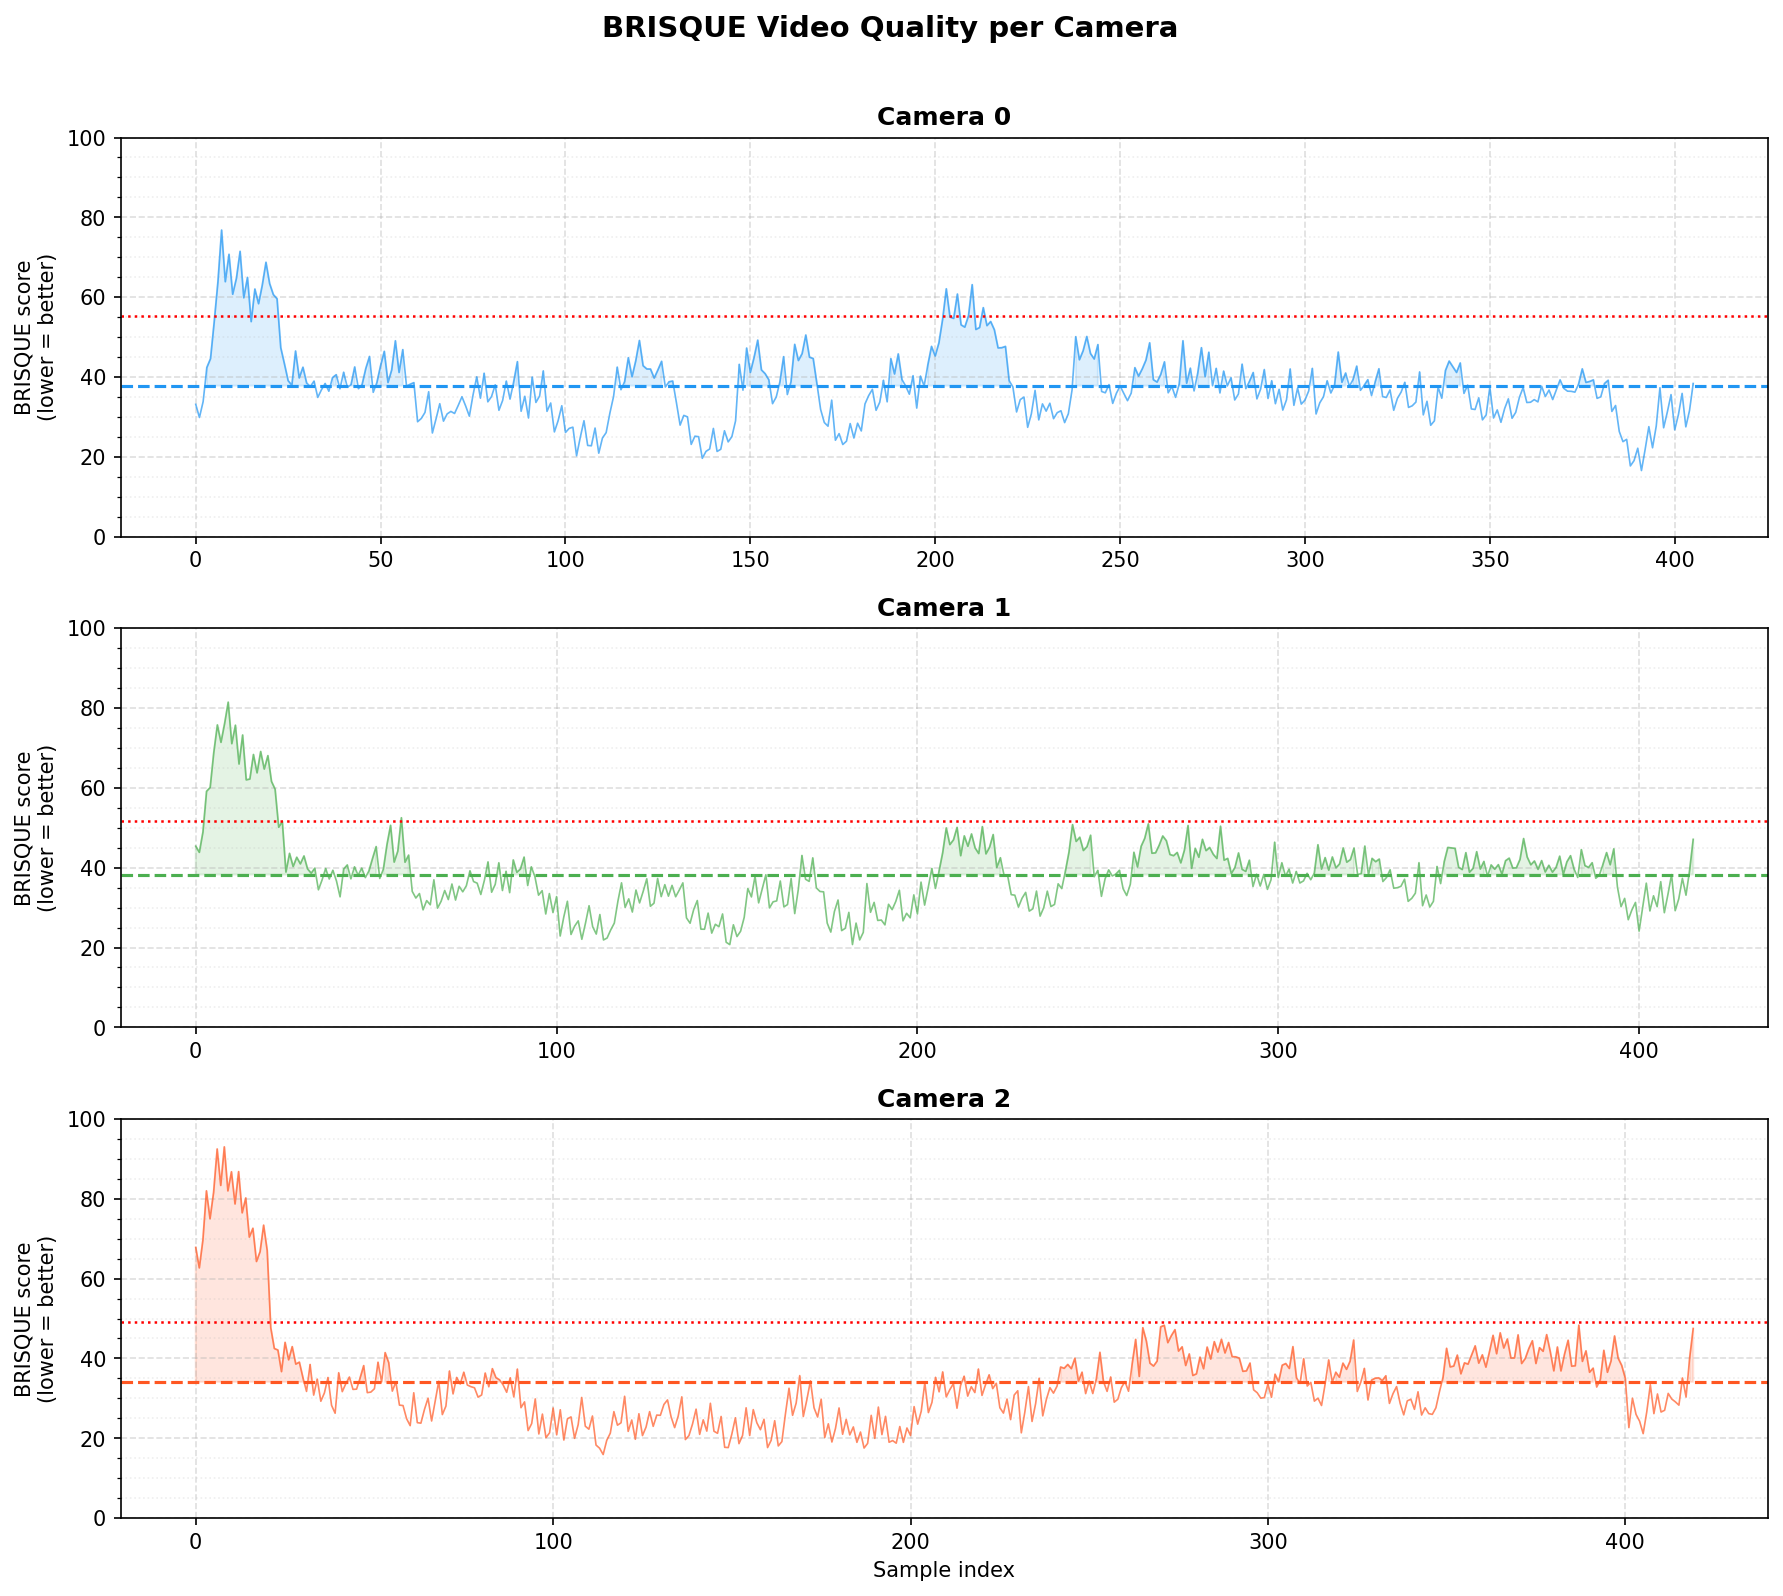
\includegraphics[width=0.95\textwidth]{Code/Analyzers/graphs/C1-26.05-09:49/quality_plot_26.05-09:49.png}
    \caption{Video Quality with BRISQUE score graph over time for C1.}\label{fig:C1Quality}
\end{figure}

Interpretation of these findings, including their implications for remote train operation and comparison against the 3GPP TS~22.289 latency threshold, is provided in Chapter~\ref{sec:discussion}.
